\subsection{Сходимость и полнота систем функций в пространствах \texorpdfstring{$C$}{C} и \texorpdfstring{$L_p$}{Lp}}


Можно построить следующую систему вложений: топологические пространства $\supset$ метрические пространства $\supset$ нормированные пространства $\supset$ предгильбертовы пространства. 

\begin{to_def}
    \textit{Банахово пространство} -- полное нормированое пространство. 
\end{to_def}

\begin{to_def}
    \textit{Гильбертово пространство} -- банахово пространство, с нормой, порожденной положительно определенным скалярным произведением $\|x\| = \sqrt{(x, x)}$.
\end{to_def}

\begin{to_def}
    \textit{Гильбертово пространство} -- \sout{полное} нормированое пространство, с нормой, порожденной положительно определенным скалярным произведением $\|x\| = \sqrt{(x, x)}$.
\end{to_def}

Приведем некоторые примеры: пространство непрерывных функций $C[a, b]$ с нормой $\|\cdot\|_C = \|\cdot\|_{\infty} = \sup_{t \in [a, b]} |x(t)|$. Пространство $L_p$. Пространство $C_p$, совпадающее с $C[a, b]$, но с нормой $\|\cdot\|_2$ -- предгильбертово, кстати.


\subsubsection*{Т1}

Построим табличку сходимостей. Для начала вспомним, что если $\mu(A) < + \infty$ и 
$1 \leq p_1 < p_2 \leq + \infty$, то
\begin{equation*}
    \|\cdot\|_{p_1} \leq C(\mu(A), p_1, p_2) \|\cdot\|_{p_2},
    \hspace{5 mm} 
    C(\ldots) = \left(\mu(A)\right)^{\frac{p_2-p_1}{p_1 p_2}}.
\end{equation*}
В частности, можно перейти к пределу, и обнаружить, что
\begin{equation*}
    \|\cdot\|_1 \leq C(\ldots) \|\cdot\|_{\infty},
    \hspace{5 mm} 
    \|\cdot\|_{\infty} = \lim_{p\to \infty} \|\cdot\|_p \equiv \|\cdot\|_C.
\end{equation*}
Таким образом из сходимости $L_2$ следует сходимость в $L_1$. 

Ещё раз напишем, что значит сходимость по норме:
\begin{equation*}
    f_n \underset{L_p}{\to} f
    \hspace{5 mm} \Leftrightarrow \hspace{5 mm} 
    \forall \varepsilon > 0 \ 
    \exists N_\varepsilon \in \mathbb{N} \ 
    \forall n \geq N_\varepsilon \ 
    \|f_n - f\|_p < \varepsilon.
\end{equation*}
Тогда рассмотрим
\begin{equation*}
    \|f_n - f\|_1 \leq \sqrt{b-a}  \|f_n -f\| < \varepsilon,  \ \qed.
\end{equation*}
Теперь докажем $f_n \underset{C}{\to} f \ \Rightarrow \ f_n \underset{L_2}{\to} f$, где сходимость по $C$-норме:
\begin{equation*}
    \forall \varepsilon > 0 \ 
    \exists N_\varepsilon \in \mathbb{N} \ 
    \forall n \geq N_\varepsilon \ 
    \forall x \in A \ 
    |f_n(x)-f(x)| < \varepsilon.
\end{equation*}
Ну, действительно,
\begin{equation*}
    \|f_n -f\|_2^2 = \int_A |f_n-f|^2(x) \mu(\d x) \leq \int_A \left\{
        \sup_{x \in A} |f_n - f|(x)
    \right\}^2 \mu(\d x) = 
    \left\{
        \sup_{x \in A} |f_n - f|(x)
    \right\}^2 \mu(A),
\end{equation*}
где множитель перед $\mu(A)$ стремится к 0 при $n \to \infty$, $\qed$. 

Также стоит вспомнить, что из равномерной сходимости следует поточечная сходимость. По определению, поточечная сходимость:
\begin{equation*}
    \forall x \in A \ 
    \forall \varepsilon > 0 \ 
    \exists N(\xi, \varepsilon) \in \mathbb{N} \ 
    \forall n \geq N \ 
    |f_n-f|(x) < \varepsilon.
\end{equation*}
Получается, что достаточно взять $N(x, \varepsilon) = N(\varepsilon)$ и получить искомое утверждение. 

В качетсве контрпримера рассмотрим $f_n(x) = n \arcctg(n/x^2)$ с $A = [1, _\infty)$. По отрицанию условия Коши, если
\begin{equation*}
    \exists \varepsilon_0 \ 
    \forall k \in \mathbb{N} \ 
    \exists n \geq k \ 
    \exists p \in \mathbb{N} \
    \exists \tilde{x} \in A \colon \ 
    |f_{n+p}-f_n|(\tilde{x}) \geq \varepsilon_0,
\end{equation*}
то последовательность $f_n$ не явдяется равномерно сходящейся. Действительно,
при $n=k$, $p=2k-2n$, $\tilde{x} = \sqrt{k} = \sqrt{n}$, верно, что
\begin{equation*}
    |f_{n+p}-f_n|(\tilde{x}) = n|2\arctg 2 - \arctg 1| \geq |2 \arctg 2 - \pi/4| = \varepsilon_0 > 0,
\end{equation*}
что говорит об отсутсвие равномерной сходимости. При этом $f_n \to x^2$ поточечно на $x \in E$. 

\textbf{Контрпримеры}. Покажем, что $f_n \underset{L_1}{\to} f \not \Rightarrow f_n \underset{L_2}{\to} f$. Прямую мы умеем строить по двум точкам
\begin{equation*}
    \frac{f-f_0}{f_1-f_0} = \frac{x-x_0}{x_1-x_0},
\end{equation*}
Построим последовательность функций вида
\begin{equation*}
    \frac{f_n - c_n}{0-c_n} = \frac{x-0}{x_n-0},
    \hspace{5 mm} 
    f_n(x) = \left\{\begin{aligned}
        &c_n(1-\textstyle \frac{x}{x_n}), &x\in[0, x_n), \\
        &0, &x\in[x_n, 1].
    \end{aligned}\right.
\end{equation*}
Контропримеры строим на отрезке $[0, 1]$. Выберем последоательность сходящуюся к $0$ в $L_1$ норме:
\begin{equation*}
    \|f_n - 0\|_1 = \int_0^{x_n} \left| 
        c_n\left(1- \textstyle\frac{x}{x_n}\right)
    \right| \mu(\d x) = \frac{1}{2} c_n x_n,
    \hspace{5 mm} 
    \|f_n - 0\|_2^2 = \frac{1}{3} c_n^2 x_n,
    \hspace{0.5cm} \Rightarrow \hspace{0.5cm}
    \|f_n\|_2 = \frac{1}{\sqrt{3}} c_n \sqrt{x_n}.
\end{equation*}
Пусть $c_n x_n = \alpha_n$ -- бесконечно малая последовательность. Выберем $x_n = 1/n$, тогда $c_n = n \alpha_n$. 

Для $\|f_n\|_2 = \frac{1}{\sqrt{3}} \frac{\alpha_n}{\sqrt{x_n}} = \frac{1}{\sqrt{3}} \sqrt{n} \alpha_n$, что устремим к $\infty$, выбрав
\begin{equation*}
    \alpha_n = \frac{1}{n^{1/2-\xi}},
    \hspace{5 mm} 
    \xi \in\left(0, \frac{1}{2}\right),
    \hspace{5 mm} 
    \qed.
\end{equation*}
Эту историю можно обобщить до отсутсвия следствия в $\|f_n\|_p = c_n x_n^{1/p} (1+p)^{-1/p}$. Тогда можем взять $\alpha_n = \left(n^{1-1/p-\xi}\right)^{-1}$, для $\xi \in (0, 1-1/p)$.

Теперь покажем, что $f_n \underset{L_2}{\to}  f \not \Rightarrow f_n \underset{C}{\to} f$. Пусть $f_n \to 0$ в $L_2$ норме. Пусть
\begin{equation*}
    \|f_n - 0\|_2 = \|f_n\| = \frac{c_n}{\sqrt{3}} x_n = \alpha_n,
    \hspace{5 mm}  x_n = \frac{1}{n}.
\end{equation*}
Пусть $f_n$ вида
\begin{equation*}
    f_n(x) = \left\{\begin{aligned}
        &\sqrt{3} \alpha_n \sqrt{n} (1-nx), &x\in[0, 1/n)
        &0, &x\in(1/n, 1].
    \end{aligned}\right. 
\end{equation*}
В таком случае
\begin{equation*}
    \sup_{x\in[0, 1]} |f_n - 0|(x) = \sup_{x\in[0, 1/n]} |\sqrt{3} \alpha_n \sqrt{n} (1-nx)| =
    \sqrt{3}  \alpha_n \sqrt{n} \not \to 0,
    \hspace{5 mm}   
    \alpha_n = \frac{1}{n^{1/2-\xi}},
    \hspace{5 mm} \xi \in[0, 1/2),
\end{equation*}
что и требовалось доказать. 

Пусть теперь есть поточечная сходимость но нет сходимости в $L_1$. Построим пилу, вида
\begin{equation*}
    f_n (x) = \left\{\begin{aligned}
        &c_n \textstyle \frac{x_{1,n}-x}{x_{1,n}-x_n}, 
        &x \in (x_{1,n}, x_n], \\
        &c_n \textstyle \frac{x_{2,n}-x}{x_{2,n}-x_n}, 
        &x \in[x_n, x_{2,n}), \\
        &0, 
        & x\in[0, x_{1,n}] \cup [x_{2,n}, 1].
    \end{aligned}\right.
\end{equation*}
В этой задаче достаточно считать $x_{1,n} = 1/(n+1)$, а $x_{2,n} = 1/n$, тогда
\begin{equation*}
    \|f_n\|_1 = c_n \frac{x_{2,n}-x_{1,n}}{2} = \frac{c_n}{2} \frac{1}{(n+1)n} \to \infty.
\end{equation*}
Чтобы это сделать, достаточно выбрать $c_n = n^{2+\xi}$. Однак поточечно такой зуб пилы сходится к $0$. Действительно, при $x=0$  $f_n(0) = 0$. Для остальных $x$ можно показать, что по определению $\lim_{n\to \infty} f_n (x) = 0$. 
\subsubsection*{Т2}


Приведем пример, когда последовательность функция $(f_n)$ сходится в пространстве $L_1[a, b]$, но для любого $x \in[a, b]$ последовательность чисел $f_n(x)$ расходится. 

Из сходимости в $L_1$ следует сходимость по мере, так что можем воспользоваться \textit{примером Рисса}. Пусть $f_n \underset{L_2}{\to}  f \equiv 0 $. Рассмотрим конструкцию вида
\begin{equation*}
    \varphi_{m,k} (x) = \xi\left[\frac{k}{2^m},\, \frac{k+1}{2^m}\right](x),
    \hspace{5 mm} 
    m \in \mathbb{N}_0,
\end{equation*}
где $k=0,1\ldots,2^{m}-1$. Утверждается, что $\forall n \in \mathbb{N} \ \exists ! m, k \ \colon  \ n = 2^m + k$. Таким нетривиальным образом мы (точнее Рисс) решили дробить ступеньку. Верно, что
\begin{equation*}
    \|f_n-0\|_1 = \int_{k/2^m}^{(k+1)/2^m} \varphi_{m ,k} (x) \d x = \frac{1}{2^m} \underset{n\to\infty}{\to} 0.
\end{equation*}
Однако, для $\forall x \in[0, 1]$ существует бесконечное число сленов последовательности равных $0$ и $1$. Таким образом поточечно последовательнсоть расходится.

\subsubsection*{Т3}

Докажем, что естественное отображение $C[a, b] \to L_1[a,b]$ не сюръективно, не забывая, что элементы $L_1$ -- это не функции, а классы эвкивалентности. 

Достаточно выбрать функцию, вида
\begin{equation*}
    f(x) = \sign x, 
\end{equation*}
которую \textit{нельзя} изменить на множестве нулевой меры, чтобы сделать её непрерывной. 
\subsubsection*{Т4}


Выясним полноты некоторых систем функций в пространстве $L_2[0,\pi/2]$. Начём с 
\begin{equation*}
    \{f_n(x) = \sin[(2n-1)x]\}_{n\in \mathbb{N}}.
\end{equation*}

\begin{to_def}
    Пусть $X$ -- нормированное пространство. Система $S = \{f_\alpha\}_{\alpha\in \mathcal A}$ называется \textit{полной}, если $\forall x \in X$ $\forall \varepsilon > 0$ $\exists \alpha_1, \ldots, \alpha_n \in \mathcal A$, а также $\exists f_{\alpha_1}, \ldots, f_{\alpha_n} \in S$ такие, что $\|x- (\alpha_1 f_{\alpha_1} + \ldots + \alpha_n f_{\alpha_n})\|_X < \varepsilon$.
\end{to_def}

Стоит подчеркнуть, что это не определение базиса, так как $\alpha \equiv \alpha(\varepsilon)$. Это определение слабее базиса, это -- приближение.

Если мы возьмём $L_2[-\pi,\pi]$, и систему вида $\{1, \sin(nx), \cos(nx)\}_{n\in \mathbb{N}}$, то она будет полна, более того будет являеться базисом. В рамках задачи мы интересуемся промежутком $[0, \pi/2]$. 

Более того, такая система полна в $\overset{\circ}{C}[-\pi, \pi],\, (f(-\pi)=f(\pi))$, чем мы потом воспользуемся в Т5.

В смысле $L_2$ мы можем приближать, игнорируя счётное число точек:
\begin{equation*}
    \|f-\tau_n\|_2^2 = \int_0^{\pi/2} |f-\tau_n| (x) \mu(\d x).
\end{equation*}
Достраивая функцию специфичным образом на отрезок $[-\pi, \pi]$ (u, d, u, d), пользуемся знанием о полноте тригонометрической системы и приходим к полной системе. 

Для понимания продолжения функции с отрезка $[0, \pi/2]$, на $[-\pi, \pi]$, достаточно построить функции, образующие системы (рис. 1). 
\begin{figure}[ht]
    \centering
    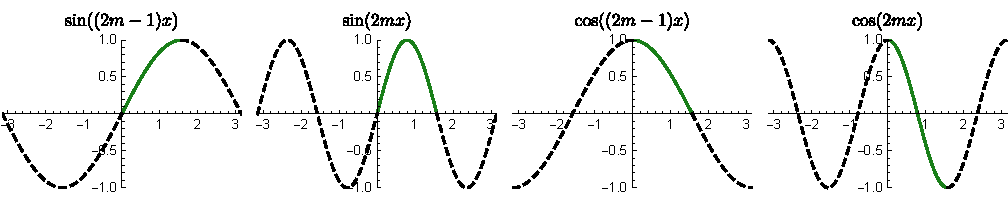
\includegraphics[width=0.8\textwidth]{figures/1.pdf}
    \caption{Графики функция при $m=1$ для Т4}
\end{figure}
И, аналогично, для $k=2$ (рис. 2). 
\begin{figure}[ht]
    \centering
    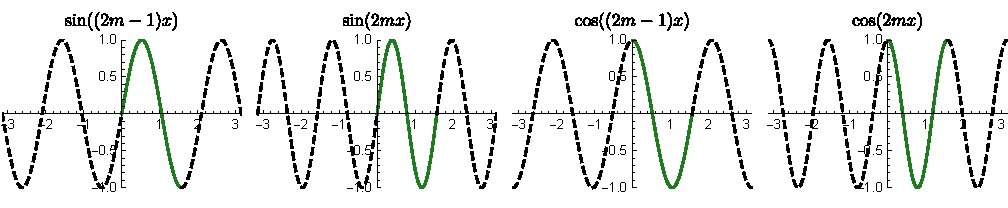
\includegraphics[width=0.8\textwidth]{figures/2.pdf}
    \caption{Графики функция при $m=2$ для Т4}
\end{figure}




\subsubsection*{Т5}

Аналогично Т4, рассмотрим полноту систем некоторых функция в пространстве $C[0, \pi/2]$. В частности покажем, что $\exists \tilde{x} \in C[0, \pi/2]$ и $\exists \varepsilon_0 \ \forall \tau_n$. Все синусы упираются в 0, выберем $\tilde{x}(t) = 1$, тогда
\begin{equation*}
    \|\tilde{x} - \tau_n\|_{\infty} = \sup_{x \in [0, \pi/2]} |\tilde{x}(t) - \tau_n(t)| \geq |\tilde{x} - \tau_n| = |\tilde{x}-\tau_n|(0) = 
    |1-0| = \varepsilon_0.
\end{equation*}
Получается, что ломаются все синусы и косинусы с <<нечётными дугами>> (достаточно взять $t=\frac{\pi}{2}$), что явно видно по построению. 

Итого, единственная хорошая система, -- $\cos(2k\, x)$. 
\subsubsection*{Т6. Функции Эрмита}

Приведем пример счетной системы фукций, полной в $L_2(\mathbb{R})$. В частности, воспользуемся функциями Эрмита:
\begin{equation*}
    \varphi_n (t) = c_n H_n(t) e^{-\frac{1}{2}t^2},
    \hspace{5 mm} 
    H_n (t) = e^{\frac{1}{2}t^2} \frac{d^n}{d t^n} e^{-\frac{1}{2} t^2}.
\end{equation*}
Утверждается, что это базис $L_2(\mathbb{R})$, докажем это. 

Есть система функций
\begin{equation*}
    \mathcal L = \{\varphi_n (t)\} = \{\rho(t) e^{-\frac{1}{2}t^2}, \ \rho \in \mathcal P\}. 
\end{equation*}
Так как $L_2$ -- гильбертово пространство, то достаточно проверить замкнутость системы, то есть показать, что $\mathcal L^\bot = \{0\}$. По определению:
\begin{equation*}
    f \in \mathcal L^\bot,
    \hspace{0.5cm} \Rightarrow \hspace{0.5cm}
    \int_{\mathbb{R}} f(t) t^n e^{-\frac{1}{2}t^2} \d t = 0,
    \hspace{5 mm} n \in \mathbb{N}. 
\end{equation*}
Рассмотрим преобразование Фурье:
\begin{align*}
    F\left[f(t)e^{-\frac{1}{2}t^2}\right](y) &= \int_{\mathbb{R}} \frac{\d t}{\sqrt{2\pi}} f(t) e^{-\frac{1}{2}t^2}, e^{-i y t} = 
    \int_{\mathbb{R}} \frac{\d t}{\sqrt{2\pi}} f(t) e^{-\frac{1}{2}t^2} 
    \sum_{n=0}^{\infty} \frac{(-iy t)^n}{n!} =\\
    &\overset{\encircled{!}}{=} 
    \sum_{n=0}^{\infty}  \frac{(-iy)^n}{n!} \int_{\mathbb{R}} \frac{\d t}{\sqrt{2\pi}} f(t) \underbrace{t^n e^{-\frac{1}{2}t^2}}_{=0 \text{\ по условию}} = 0,
\end{align*}
таким образом мы выяснили, что Фурье функции $\equiv 0$. 

Далее воспользуемся тем, что $f(t) e^{-\frac{1}{2}t^2} \in L_2\left(\mathbb{R}\right)$, а значит работает равенство Парсеваля:
\begin{equation*}
    \int_\mathbb{R} \bigg|f(t) e^{-\frac{1}{2}t^2}\bigg|^2 \frac{\d t}{2 \pi} = 
    \int_{\mathbb{R}} \big|F[\ldots](y)\big|^2 \d y = 0,
    \hspace{0.5cm} \Rightarrow \hspace{0.5cm}
    f(t) e^{-\frac{1}{2}t^2} = 0,
    \hspace{0.5cm} \Rightarrow \hspace{0.5cm}
    f(t) = 0,
\end{equation*}
по крайней мере кроме множества меры нуль. Таким образом функции эрмита составляют базис в $L_2$.



% \encircled{!} -- теоерма Фубини, объяснить, лемма Лебеша о мажорируемой сходимости


\subsubsection*{Т7}


Возьмём функцию, которая лежит в $L_2$, но не лежит в $
\overset{\vspace{-1pt}\scalebox{0.5}{$\circ$}}{C} [-\pi,\pi]$, например, ограничение $\sign x$. И рассмотрим
подпространство $V\subset \overset{\vspace{-1pt}\scalebox{0.5}{$\circ$}}{C} [-\pi,\pi]$, заданное ортогональностью к
ней, то есть заданное формулой
\[
\int_{-\pi}^0 f(x)\; dx = \int_0^\pi f(x)\; dx.
\]

Это $V$ есть замкнутое подпространство в $\overset{\vspace{-1pt}\scalebox{0.5}{$\circ$}}{C}[-\pi,\pi]$ и в нём
можно выбрать какую-то полную систему, и даже её ортогонализовать. Если
начать с тригонометрической системы, то косинусы и чётные синусы и так
лежат в $V$, нечётные синусы надо будет подправить, скомбинировав их с
$\sin x$, а потом ещё ортогонализовать (что может быть неприятно).

В итоге, система не может быть полна в $\overset{\vspace{-1pt}\scalebox{0.5}{$\circ$}}{C}[-\pi,\pi]$, так как её
линейные комбинации не выходят за пределы $V$. А что касается
замкнутости, то переходя в гильбертово $L_2$ видно, что ортогональное
дополнение к замыканию образа $V$ в гильбертовом пространстве одномерно
и натянуто на этот вот $\sign x$, который разрывен и не лежит в образе
$\overset{\vspace{-1pt}\scalebox{0.5}{$\circ$}}{C}[-\pi,\pi]$. Так что замкнутость в терминах $\overset{\vspace{-1pt}\scalebox{0.5}{$\circ$}}{C}[-\pi,\pi]$ есть.
